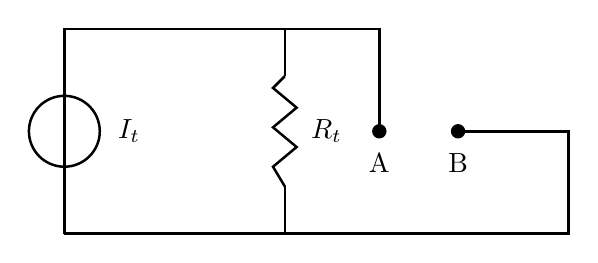
\begin{tikzpicture}[line width=0.9pt]
  % left branch: current source I_t
  \draw (0,0) -- (0,2.6) -- (2.8,2.6);
  \draw (0,0) -- (2.8,0);
  \draw (0,1.3) circle (0.45);
  \node[right] at (0.55,1.3) {$I_t$};
  % middle branch: variable resistor R_t (zigzag with arrow)
  \draw (2.8,2.6) -- (2.8,2.0);
  \draw (2.8,0)   -- (2.8,0.6);
  \draw (2.8,2.0) -- (2.65,1.85) -- (2.95,1.6) -- (2.65,1.35)
        -- (2.95,1.1) -- (2.65,0.85) -- (2.8,0.6);
  \node[right] at (3.0,1.3) {$R_t$};
  % terminals A and B
  \fill (4.0,1.3) circle (2.6pt);
  \fill (5.0,1.3) circle (2.6pt);
  \node[below] at (4.0,1.15) {A};
  \node[below] at (5.0,1.15) {B};
  % wiring: top rail to A, B out to right and back to bottom rail
  \draw (2.8,2.6) -- (4.0,2.6) -- (4.0,1.3);
  \draw (5.0,1.3) -- (6.4,1.3) -- (6.4,0) -- (2.8,0);
  % outer frame corners already drawn; connect top-left up node
\end{tikzpicture}
